%%%%%%%%%%%%%%%%%%%%%%%%%%%%%%%%%%%%%%%%%%%%%%%%%%%%%%%%%%%%%%%%%%%%%%%%%%%%%%%%
% ---------------------------------------------------  ADD HERE YOUR REPORT  ---
%%%%%%%%%%%%%%%%%%%%%%%%%%%%%%%%%%%%%%%%%%%%%%%%%%%%%%%%%%%%%%%%%%%%%%%%%%%%%%%%

%sources:
% 0: https://arxiv.org/pdf/1006.1718v2.pdf





\section{Introduction}
\label{sec:intro}

The aim of this theses is to determine the concentration of \nuc{Kr}{85} in the liquid argon coolant and scintillator of the GERDA experiment and by this determining its influence on the radioactive background. 

The GERDA experiment tries to find evidence for the existence of the neutrino less double beta decay in \nuc{Ge}{67} as it was reported to be found in the NAMEDESANDERENEXPERIMENTSHIER. Because it is expected that this decay has a very long lifetime it is very important to filter out every source of background radiation as good as possible. Therefor it is necessary to cool the \nuc{Ge}{67} detectors down to reduce thermal activities and have some kind of scintillator around the detectors to filter out radiation coming from outside. In this setup are the detectors also the \nuc{Ge}{67} used as radiation source which makes any signal coming from  the outside a background event. Liquid argon fits perfectly for both of theses requirements due to its low freezing point and its ability to scintillate. The majority of the impurity of the liquid argon can be removed by cryogenic distillation but even the remaining alien isotopes are still very active.\\

One of these residual radioactive isotopes is \nuc{Kr}{85}. Compared to \nuc{Ge}{67} it has a relatively low endpoint energy and therefor shouldn't create any fake neutrino less double beta decays. It also isn't the strongest radioactive background source. This title belongs to \nuc{Ar}{42}. 

% what is the general aim of my Bachelor thesis
% general overview of how I'm going to do this
% ? what are my predictions ?
% What possible influence would the result of my work might have on the result of the GERDA experiment?

\section{Physical Background}
\label{sec:PhyBG}

\subsection{Weyl, Majorana and Dirac fermions}
\label{sec:WMDf}

% in this chapter almost everything from source 0

\begin{itemize}
\item historic introduction of question whether neutrinos are dirac or majorana fermions
\begin{itemize}
\item from Dirac relativistic equation fermion fields
\item electrons: have mass and charge, Dirac-eq predicts antiparticles, requires 4-comp fields
\item Weyl calculates for massless fermions that only two-component fields are necessary
\item Pauli predicts neutrinos in letter, no charge, seems to have vanishing mass 
\item \(\rightarrow\) assumption: neutrinos  are Weyl fermions
\item Majorana: neutrinos are antiparticles of itself since they are uncharged, first not taken seriously, only after first indications that neutinos have mass
\item \(\rightarrow\) discussion whether neutrinos are Dirac or Majorana fermions
\end{itemize}
\item short introduction to dirac-eq
\begin{itemize}
\item \((i\hbar\gamma^\mu \partial_\mu  - mc)\psi = 0\) , maybe Hamilton/Lagragian, has plane waves as solution multiplied with spinor
\item Spinors: any column like function of energy and momentum which when multiplied by factor \(\exp(i\vec{p}\cdot\vec{x})\) or  \(\exp(\-i\vec{p}\cdot\vec{x})\) becomes a solution of the Dirac equation
\end{itemize}
\item we know that the Klein-Gordon-eq is real, how can we get a real solution from the dirac-eq
\begin{itemize}
\item depends on how we choose our \(\gamma^\mu\), if all non-zero elements of all the \(\gamma^\mu\) are purly imaginary, then Dirac-eq is real
\item Majorana matrices, with usage in Dirac-eq one can obtain real solutions that satisfy \(\tilde{\psi} = \tilde{\psi}^*\)
\item \(\rightarrow\) these solutions represent Majorana fermions
\item general solution to Majorana condition can be obtained by transformation with unitary matrix: \(\gamma^\mu = \mathrm{U}\tilde{\gamma^\mu}\mathrm{U}^\dagger\)
\item general Majorana condition: \(\psi = \mathrm{U}\mathrm{U}^\top\tilde{\psi}^*\), with \(\mathrm{U}\mathrm{U}^\top \equiv \gamma^0 \mathrm{C}\)
\item with compact notation \(\widehat{\psi} \equiv \gamma^0 \mathrm{C} \psi^*\)
\item general definition of a Majorana fermion fields through definition: \(\psi = \widehat{\psi}\), condition is Lorenz invariant
\end{itemize}
\item clunky repetition of what helicity and chirality is and what their problem with massive fermions is
\begin{itemize}
\item helicity defined as twice the value of the spin component of the particle along the direction of the momentum \(h_{\vec{p}} = \frac{2 \vec{J} \cdot \vec{p}}{p}\)
\item eigenstates of eigenvalue -1 called "left-helical", eigenstates of eigenvalue +1 called "right-helical"
\item is invariant under time/rotation, not invariant under boost
\item chirality meaning assigned to matrix \(\gamma_5 = i\gamma^0\gamma^1\gamma^2\gamma^3\)
\item projection matrices on fermion fields: \( \mathrm{L} = \frac{1}{2} \left( 1- \gamma_5\right ) \), \( \mathrm{R} = \frac{1}{2} \left( 1 + \gamma_5\right ) \)
\item projections of L, R are called lift/right-chiral
\item wavefunction can be written as \(\psi = \psi_L + \psi_R\) with \(\psi_L = \mathrm{L}\psi\) and \(\psi_R = \mathrm{R}\psi\)
\item \(\rightarrow\) helicity: conserved for free particles, not under Lorenz trafo
\item \(\rightarrow\) chirality: is Lorenz invariant, not conserved
\item \(\rightarrow\) both not appropriate for characterizing a fermion that has mass
\end{itemize}
\item how to define Weyl fermions
\begin{itemize}
\item problem with helicity/chirality disappears if the fermion is massless
\item general solution of Dirac-eq is not irreducible representation of Lorentz group (Lorenz group: group of Lorentz trafo in Mirkowski-space-time)
\item \(\rightarrow\) left/right-chiral fields are Lorentz invariant, representation with 2-component-field: \( \begin{pmatrix}\frac{1}{2} \\ 0\end{pmatrix}\) for left-chiral, \(\begin{pmatrix}0 \\ \frac{1}{2}\end{pmatrix}\) for right-chiral
\item when \(\chi\) is left chiral Weyl fermions, \( \widehat{\chi} \) is a right chiral Weyl fermions
\item a general fermion field can be described by two Weyl fields \(\rightarrow\) building blocks
\end{itemize}
\item how can we build Majorana/Dirac fermions from Weyl fermions
\begin{itemize}
\item Majorana and Dirac fermions both have mass and therefor must have both left/right chiral components
\item Dirac can be created by two independent left chiral Weyl fields \(\chi_1\), \(\chi_2\): \(\psi = \chi_1 + \widehat{\chi_2}\)
\item Dirac fermions are unconstrained solutions of the Dirac equation
\item unlike the Dirac fermions, the Majorana fermions must fulfill the reality condition \( \psi = \widehat{\psi} \)
\item Majorana fermions are represented by: \( \psi = \chi + \widehat{\chi} \)
\item where does mass come from?: mass term in Dirac-eq is of from \(\bar{\psi}\psi\), only \(\bar{\psi_L}\psi_R\) and \(\bar{\psi_R}\psi_L\) remains, \(\bar{\psi_L}\psi_L\) and \(\bar{\psi_R}\psi_R\) cancel out
\item \(\rightarrow\) Weyl fermions has special chirality therefore mass term must vanish, massive fermions must have left-chiral and right-chiral components
\end{itemize}
\item Dirac fields are completely unconstrained solutions of Dirac equation
\item Weyl/Majorana fields are simpler solutions with some kind of constrained imposed on solution, Weyl: chirality condition, Majorana: reality condition
\end{itemize}
% hier muss ich mich ein wenig einlesen ... mögliche Literatur:
% KTA-Expert script
% 0: https://arxiv.org/pdf/1006.1718v2.pdf

\subsection{Neutrinoless Double Beta Decay}
\label{sec:NDBD}
\begin{itemize}
\item Neutrino Oscillation have shown that neutrinos have finite mass, with NeOs only difference in mass measurable, lower limit on absolute mass with \(\mathrm{m}_{scale} = \sqrt{\Delta \mathrm{m}^2}\)
\begin{itemize}
\item SuperKamiokande showed mixing between \(\nu_\mu\) and \(\nu_\tau\) of atmospheric neutrinos
\item "solar neutrino puzzle" solved with mixing of \(\nu_e\) and mixture of \(\nu_\mu\) and \(\nu_\tau\)
\item NeOs can not determin absolute masses and also not separate between two different scenarios:
\begin{itemize}
\item hierarchical pattern ( \(m_i\)  ~= \(\sqrt{\Delta m^2}\))
\item degenerate pattern ( \(m_i >> \sqrt{\Delta m^2}\))
\end{itemize}
\end{itemize}
\item \(\beta\beta(0\nu)\) decay can only proceed when Neutrinos are massive Majorana particles
\begin{itemize}
\item standard electroweak model postulates that neutrinos are massless and total lepton number is conserved -> with \(\beta\beta(0\nu)\) physics beyond SM
\item double beta decay is rare transition between two nuclei with the same mass number A involving change of nuclear charge Z by two units
\begin{itemize}
\item can only proceed if initial nucleon is less bound than final and both are more bound than intermediate nucleon -> only fulfilled for even-even nucleons
\item \(\beta\beta(2\nu)\): \( (Z,A) \rightarrow (Z + 2, A) + e^-_1 + e^-_2 + \bar{\nu_{e1}} + \bar{\nu_{e2}} \), conserves lepton number
\item \(\beta\beta(0\nu)\): \( (Z,A) \rightarrow (Z + 2, A) + e^-_1 + e^-_2\), violates lepton number conservation
\item \(\beta\beta(0\nu, \chi)\): \((Z,A) \rightarrow (Z + 2, A) + e^-_1 + e^-_2 + \chi \)
\end{itemize}
\item easy to distinguish the three decay modes by shape of \(e^-\)-sum energy spectrum
\begin{itemize}
\item 2\(\nu\): broad maximum below half of endpoint
\item 0\(\nu\): \(e^-\) carry full available kinetic energy, single peak at endpoint
\item 0\(\nu,\chi\): again continuous, maximum shifted above halfway point
\end{itemize}
\end{itemize}
\item Majorana, Dirac neutrinos (again from above, maybe move stuff there)
\begin{itemize}
\item Majorana: particles that are identical with their own antiparticles, two component objects
\item Dirac: one can distinguish, four component objects
\item massive fermions usually described by Dirac eq with coupling of chiral eigenstates \(\psi_L,\psi_R\), \(\Psi = \begin{pmatrix} \psi_R \\ \psi_L\end{pmatrix}\)
\item Majorana suggested alternative description of massive fermions which do not have additive quantum numbers as two component states, chiral eigenstates connected via \(\psi_L = \epsilon \psi_R^*\)
\end{itemize}
\item Lorentz invariant mass in Dirac Lagrangian:
\begin{itemize}
\item Dirac mass: \(M_D [\bar{\nu_R}\nu_L + (\bar{\nu_L})^*\nu_R^*]\), requires both chirality eigenstates, conserves total lepton number
\item Majorana mass: \(M_L [(\bar{\nu_L})^*\nu_L + \bar{\nu_L}\nu_L^*]\), \(M_L [(\bar{\nu_R})^*\nu_R + \bar{\nu_R}\nu_R^*]\), violates total lepton number conservation, can be present even w/o existents of \(\nu_L/\nu_R\)
\item generally all three terms may coexist, when Lagrangian is diagonalized the resulting two general non-degenerate mass eigenvalues for each flavor (see-saw: light and heavy particle for each flavor) \(M = \begin{pmatrix} M_L & M_D \\ M_D & M_R\end{pmatrix}\) 
\item M diagonalized by unitary matrices \(\begin{pmatrix} U \\ V \end{pmatrix}\), U,V general mixing matrices, if non of the \(\nu_R\) states exist or \(M_R\) is so large only \(M_L\) is relevant and only U needed
\end{itemize}
\item Majorana mass
\begin{itemize}
\item transition amplitude for Majorana neutrino mass \(m_e\) is sum over product of \(m_j\) and combination of nuclear mixing element
\item in each vertice electron is emitted, therefor mixing amplitude \(\mathrm{U}_{ej}\) appears in each of them
\item \(\Rightarrow \beta\beta(0\nu)\) decay amplitude contains factor \(\mathrm{U}_{ej}^2\) not \(|\mathrm{U}_{ej}|^2 \Rightarrow <m_\nu> = |\sum_jm_j\mathrm{U}_{ej}^2|\) 
\end{itemize}
\item oscillation parameters
\begin{itemize}
\item \(<m_\nu>^2 = |\sum_jm_j\mathrm{U}_{ej}^2|^2 = |\sum_jm_j|\mathrm{U}_{ej}|^2e^{i\alpha}|^2\) with \(\alpha\) being the Majorana phase
\item possibility of cancellation of sum (Zee model \(<m_\nu> = 0\))
\item \(<m_\nu> = 0\) depends on unknown phase but upper/lower limit only depends on absolute values of mixing angles\(<m_\nu> = \sum_jm_j|\mathrm{U}_{ej}|^2\)
\item when \(<m_\nu>\) is known from tritium beta decay experiments one can determine phase \(\alpha_i\)
\end{itemize}
\end{itemize}

% also a bit about standard double beta decay
% differences between the standard and neutrinoless beta decay
 
\subsection{LAr as coolant} 
\label{sec:LArcoolant}



% 

\subsection{\nuc{Kr}{85} isotop}
\label{sec:Kry85}




% where does it come from?
% what properties does it have?
% why is it important to calculate its influence on GERDA

\section{GERDA}
\label{sec:GERDA}

% general Information, e.g. 
% sizes 
% Gran Sasso, 
% what other  neutrino less beta decay experiments are there,

\subsection{Aim of \GERDA}
\label{sec:AimGERDA}

% not sure whether this is enough for its own section, maybe just connect it with general info

\subsection{Experimental Setup}
\label{sec:ExSetup}

% well, just dump everything here

\subsection{Background Reduction}
\label{sec:BGReduction}

% Mui, Mountain, Pulse shape disc.
% especially LAr-Veto 

\subsection{Results}
\label{sec:ResultsofGERDA}

% what has happened so far

\section{Analysis of the \nuc{Kr}{85} concentration}
\label{sec:AotKr}

The main goal of this theses is to approximate the concentration of the isotope \nuc{Kr}{85} in the liquid argon coolant and scintillate of the GERDA. This value is of special interest, as in other experiments this isotope in the liquid argon has produced a not negligible background. For example, an activity of \((2.05\pm0.13) \mathrm{\frac{mBq}{kg}}\) was measured in the Darkside experiment \cite{PhysRevD.93.081101} and an activity of \((0.16\pm0.13)\frac{Bq}{l}\) in the WARP experiment \cite{Benetti:2006az}. 

\subsection{Different Approaches to calculate the concentration}
\label{sec:Appro}

The aim of this section is to give a rough impression of the two methods used in this theses to determine the concentration of \nuc{Kr}{85} in the liquid argon.\\

The first method for determining the concentration uses \nuc{Kr}{85}'s property to decay into an excited state of \nuc{Rb}{85} with a probability of 0.43\%. This state has a raised energy level of 514keV compared to its ground state and this excited state has a half-life of 1.015\(\mu\)s. Theoretically it should now be possible to measure a peak in the range around 514keV. Using a Monte-Carlo simulation one can also determine a function of amplitude of such a peak in the phase diagram only depending on the homogeneous concentration of \nuc{Kr}{85} in the liquid argon. Using this and the previously measured amplitude one should be able to calculate the concentration of \nuc{Kr}{85}.\\

The biggest problem of this method to overcome lies with the proximity of the \nuc{Kr}{85} to the 511keV peak of the positron electron annihilation. Its peak is expected to partially dominate over the \nuc{Kr}{85} in the phase diagram and does not allow for a direct measurement of the 514keV peak. 

%It is hoped that almost all of the positron electron annihilation events can be filtered out by only using those signals that didn't trigger LAr veto. The majority of the \nuc{Kr}{85} decay events will probably pass this filter  
%Hier halt drinnen weil iwie die Signale des Kr85 in den PMs nicht wirklich erkennbar ist und anscheinend die meisten gemessenen Events durch den Filter kommen ?!?!?!?!


The second method uses the reduction in event rate over the range of 200 to 500 keV. This is only useable because every other isotope we know that is present in the liquid argon with a non negligible proportion has a half-life much higher than \nuc{Kr}{85} with its \(10.739\mathrm{y}\). The dominant background sources are in descending order \nuc{Ar}{42} with a half-life of 32.9 y, \nuc{Ar}{39} with 269 y and \nuc{U}{232} with 68.9 y. Since the liquid argon has not been replaced since the beginning of GERDA Phase I in 2013, it can be estimated that the Kr85 rate has decreased by a factor of \(\sqrt{2}\) while the rate of the other isotopes should have hardly changed.\\

Due to routine check-ups and improvements to the experimental setup there were several time intervals in which the detector was deactivated. This means that one has to find a way to weigh the measured rates with a signal that corresponds to the times the detector was actually active. Luckily the test pulse can be used as such a reference. This test pulse emits a strong signal of TESTPULSERENERGIEHIER every twenty seconds and every measured event of it is separately marked as a test pulse signal. These signals can now be used as weigh to correct to previous histogram to get a corrected diagram. By laying a fit function of an exponential decrease plus a constant background over it one should be able to deduct the activity of the \nuc{Kr}{85} from the amplitude of the exponential decrease. With this one can then calculate the concentration by integrating over the activity and dividing over the liquid argon volume.\\

Because the second method is based on a very broad approximation it is expected to only give one a rough estimation of the actual concentration. In contrast, the first method is expected to wield a much better appraisal because it does not heavily rely on any approximation. 

%The only two places where there have been simplifications are the Monte-Carlo simulation and the homonymity approximation of the concentration of \nuc{Kr}{85} in the liquid argon. -- was ist mir LAr-Veto, weil eigentlich haben wir ja auch Kr85 zerfälle die das veto triggern während der größte Teil es nicht macht.



% short outline of approaches

\subsection{Concentration from the 514keV peak}
\label{sec:SAfrom514}


% calculate Amplitude of Gauss peak at 514keV and use factor from Monte Carlo Simulation to estimate

% look at phase diagram at range of 500 to 525 keV, use different filters and fit remaining data with Gaussian function
% -> get amplitude
% make a Monte Carlo simulation to estimate actual Kr85 activity in LAr from measured activity in detectors
% -> with amplitude and factors from MC-Simulation one can calculate the specific activity

\subsection{Concentration from the decrease in rate}
\label{sec:SAfromDecrease}

% use fit to calculate the decrease in rate of the signals in range from 200 to 500keV
% from fit and assumption that only Kr85's activity is decreasing one can calculate the specific activity from the amplitude of the fit

% use Volume of LAr-Tank to determine the number of Kr85 and from this the concentration in the argon

\section{Conclusion}

% what went wrong?
% what does it mean?
% possible future enhancements to determine the Kr85 concentration

































% %%%%%%%%%%%%%%%%%%%%%%%%%%%%%%%%%%%%%%%%%%%%%%%%%%%%%%%%%%%%%%%%%%%%%%%%%%%%%%%%
% \section{Another Section}
% \label{sec:secname}


% Fig.~\ref{fig:pmt} shows a PMT.

% %------------------------------------------------------------------- figure ----
% \begin{figure}[hb]
% \centering
% \ifmakefigures%
%    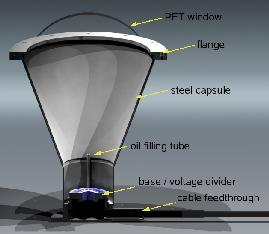
\includegraphics[width=45mm]{kapselung-small.jpg}
% \fi%
%   \caption{\label{fig:pmt}
% The encapsulation of the Cerenkov PMT.
% }
% \end{figure}
% %-------------------------------------------------------------------------------

% %%%%%%%%%%%%%%%%%%%%%%%%%%%%%%%%%%%%%%%%%%%%%%%%%%%%%%%%%%%%%%%%%%%%%%%%%%%%%%%%
% \section{Results and Analysis}
% \label{sec:results}


% %----------------------------------------------------------------- equation ----
% {\centering
% \begin{equation}\label{eq:sensit}
%     T_{1/2}(0^{+} \rightarrow g.s.~with~single~\gamma)~ \geq ~\ln2 \cdot
%     \varepsilon \cdot a \cdot \frac{M \cdot N_A}{A} \cdot 
%     \sqrt{\frac{\Delta T}{b\cdot\Delta E}},
% \end{equation}
% } % end centering
% %-------------------------------------------------------------------------------

% Table~\ref{tab:param} compiles everything.

% %-------------------------------------------------------------------- table ----
% \begin{table}[t]
% \centering
% \caption{\label{tab:param}
% Experimental parameters and values.
% }
% \vspace*{2mm}
% \begin{tabular}{L{4cm}|C{6cm}}
%   Column1 & Column2 \\  \hline 
%   Row1 & $100\pm10$ \\
%   Row2 & $100\pm10$ \\ \hline
%   Row3 & $100\pm10$ \\
%   Row4 & $100\pm10$ \\ 
% \end{tabular}
% \end{table}
% %-------------------------------------------------------------------------------

% %%%%%%%%%%%%%%%%%%%%%%%%%%%%%%%%%%%%%%%%%%%%%%%%%%%%%%%%%%%%%%%%%%%%%%%%%%%%%%%%
% \section{Conclusions}
% \label{sec:conclusions}
